% !TEX TS-program = pdflatex
% !TEX encoding = UTF-8 Unicode

% This is a simple template for a LaTeX document using the "article" class.
% See "book", "report", "letter" for other types of document.

\documentclass[14pt]{article} % use larger type; default would be 10pt

\usepackage[utf8]{inputenc} % set input encoding (not needed with XeLaTeX)

%%% Examples of Article customizations
% These packages are optional, depending whether you want the features they provide.
% See the LaTeX Companion or other references for full information.

%%% PAGE DIMENSIONS
\usepackage{geometry} % to change the page dimensions
\geometry{a4paper,total = {170mm , 257 mm},left = 40mm,top=35mm,right = 30mm,bottom=15mm,} % or letterpaper (US) or a5paper or....
% \geometry{margin=2in} % for example, change the margins to 2 inches all round
% \geometry{landscape} % set up the page for landscape
%   read geometry.pdf for detailed page layout information

\usepackage{graphicx} % support the \includegraphics command and options
\usepackage{mdframed}

% \usepackage[parfill]{parskip} % Activate to begin paragraphs with an empty line rather than an indent
\usepackage{float}
\usepackage{titling}
\usepackage{subcaption}
\setlength{\parindent}{4em}
%%% PACKAGES
\usepackage{booktabs} % for much better looking tables
\usepackage{array} % for better arrays (eg matrices) in maths
\usepackage{paralist} % very flexible & customisable lists (eg. enumerate/itemize, etc.)
\usepackage{verbatim} % adds environment for commenting out blocks of text & for better verbatim
%\usepackage{subfig} % make it possible to include more than one captioned figure/table in a single float
% These packages are all incorporated in the memoir class to one degree or another...

%%% HEADERS & FOOTERS
\usepackage{fancyhdr} % This should be set AFTER setting up the page geometry
\pagestyle{fancy} % options: empty , plain , fancy
\renewcommand{\headrulewidth}{1pt} % customise the layout...
\lhead{}\chead{}\rhead{Project Report | DRDO}
\lfoot{}\cfoot{}\rfoot{\thepage}
\topmargin = -23pt
\headsep = 10pt
\renewcommand{\footrulewidth}{1pt}

%%% SECTION TITLE APPEARANCE
\usepackage{sectsty}
\allsectionsfont{\sffamily\mdseries\upshape} % (See the fntguide.pdf for font help)
% (This matches ConTeXt defaults)

%%% ToC(table of contents) APPEARANCE
\usepackage[nottoc,notlof,notlot]{tocbibind} % Put the bibliography in the ToC
\usepackage[titles,subfigure]{tocloft} % Alter the style of the Table of Contents
\usepackage{amsmath}
\usepackage{lmodern}
\usepackage{tcolorbox}
\usepackage{indentfirst}
\usepackage{changepage}
\renewcommand{\cftsecfont}{\rmfamily\mdseries\upshape}
\renewcommand{\cftsecpagefont}{\rmfamily\mdseries\upshape} % No bold!

%%% END Article customizations

%%% The "real" document content comes below...



%\date{} % Activate to display a given date or no date (if empty),
         % otherwise the current date is printed 

\begin{document}
\tableofcontents
\listoffigures
\pagebreak
\title{CHAPTER 1}
\maketitle
\section{INTRODUCTION}

\subsection{INTRODUCTION}
         Radar systems are generally used in determining properties, most commonly distance from a reference point, of solid objects using single antennas or large antenna arrays. These antennas transmit and receive electromagnetic signals, which can be processed to obtain various relevant data. By using only one antenna and moving it along a linear axis to record an area of static objects, one can mimic a larger array of antennas to collect high-resolution data: this setup is known as a synthetic aperture radar system. The data collected from this type of radar configuration, after processing, is well-known for its detail and map-like quality, and can be used to render a two-dimensional and three-dimensional representation of scanned area.

\subsection{PROBLEM STATEMENT}
           Radars produce large amounts of data and this has important implications for the archiving and analysis of data. The need for methods to deal with radar data sets will only increase as DRDO is developing multiple sided radar under their project QRSAM. Till now Radar data has been processed in a very traditional manner by going through each bit of big binary files. So, each time whenever an information about particular dwells were needed, it involved a long task of searching each binary files and getting the information. Also the raw radar data contain lot of garbage data which makes it difficult and tedious task to test radar during its development phase. The brute force approach of reading data every time when needed from raw files, uncompressing the data, analysing, loading another chunk, and so on, is impractical. For one, it limits access to the data and prevents parallel research activities.

\subsection{OBJECTIVE}
 To develop a software capable of handling large raw binary radar data and reading each dwells and saving information in a database. Also the software should be capable of reading multiple data without any loss in dwells information and can exclude garbage data. The software should be able to extract clean required radar data and merge it to files. The final objective of this project includes its analysis and the algorithm devised should be fast enough to process large data at real time. 
 \subsection{LITERATURE SURVEY}
 The subject of Radar data logger is an active research area due to change in computer technologies and evolving software tools.
 \begin{itemize}
 \item In [1],author suggested and used MATLAB to process raw radar data produced from simulators like ISARLAB ( A simulator for high resolution radar data) which uses brut force method to read the data from raw binary files and then the binary file is converted into MATLAB binary format for its analysis.
 \item In[2],author made a software which uses MATLAB for core processing and analysis of raw radar data at real time. To read data and its header from multiple files and its analysis, it used burst plot method in which if modification file is read the next time and same data file is opened, the already plotted burst will not be plotted again in the display plot.
 \item In[3],author desribe the use of microprocessor to read the raw radar binary files and remove garbage and store high resolution data in SD card for further processing.
 \item In[4],author proposes the use of database for automatic target recognition by gathering data in database and using the database for automatically detecting target.
 \item In[5], analysis of traffic radar is done by using database and softwares which plots the data from the database on daily basis to help the government for analysing traffic in the city.
 \end{itemize}

\subsection{HARDWARE USED}
\noindent The hardware used in this project are :\\
\textbf{Processor : } \\
\indent Intel (R) Xeon (R) CPU E5 - 2660, 2.20GHz\\
\\ \textbf{Installed Memory : }\\
\indent 16.0 GB\\
\\ \textbf{System Type : }\\
 \indent 64-bit Architecture
 
 \subsection{SOFTWARE USED}
 \noindent The software used in this project are :\\
\\ \indent \textbf{Database :}\\
\indent MS SQL 2008 R2 \\ \par
  SQL Server Management Studio (SSMS) is a software application first launched with Microsoft SQL Server 2005 that is used for configuring, managing, and administering all components within Microsoft SQL Server. The tool includes both script editors and graphical tools which work with objects and features of the server.
A central feature of SSMS is the Object Explorer, which allows the user to browse, select, and act upon any of the objects within the server. It also shipped a separate Express edition that could be freely downloaded, however recent versions of SSMS are fully capable of connecting to and manage any SQL Server Express instance. Microsoft also incorporated backwards compatibility for older versions of SQL Server thus allowing a newer version of SSMS to connect to older versions of SQL Server instances.\\  \par
\textbf{Editor :}\\
\indent Visual Studio 2008 version 9.0.30\\ \par
Microsoft Visual Studio is an integrated development environment (IDE) from Microsoft. It is used to develop computer programs for Microsoft Windows, as well as web sites, web apps, web services and mobile apps. Visual Studio uses Microsoft software development platforms such as Windows API, Windows Forms, Windows Presentation Foundation, Windows Store and Microsoft Silverlight. It can produce both native code and managed code.
Visual Studio includes a code editor supporting IntelliSense (the code completion component) as well as code refactoring. The integrated debugger works both as a source-level debugger and a machine-level debugger. Other built-in tools include a code profiler, forms designer for building GUI applications, web designer, class designer, and database schema designer. It accepts plug-ins that enhance the functionality at almost every level—including adding support for source control systems (like Subversion) and adding new toolsets like editors and visual designers for domain-specific languages or toolsets for other aspects of the software development lifecycle (like the Team Foundation Server client: Team Explorer).\\  \par
\textbf{Analysis Software :}\\
\indent MATLAB R2009a\\ \par
MATLAB (matrix laboratory) is a multi-paradigm numerical computing environment and fourth-generation programming language. A proprietary programming language developed by MathWorks, MATLAB allows matrix manipulations, plotting of functions and data, implementation of algorithms, creation of user interfaces, and interfacing with programs written in other languages, including C, C++, C\#, Java, Fortran and Python.
Although MATLAB is intended primarily for numerical computing, an optional toolbox uses the MuPAD symbolic engine, allowing access to symbolic computing abilities. An additional package, Simulink, adds graphical multi-domain simulation and model-based design for dynamic and embedded systems.

 
 \subsection{TECHNOLOGY STACK}
\noindent The technology and languages used in this project are :
\subsubsection{Back-end Technology Stack}
\indent \textbf{SQL - } used for storing, accessing and retrieving various data across database.\\
\\ \indent \textbf{C\# - } used for coding, connectivity, business logic generation and execution part.
\subsubsection{Fron-end Technology Stack}
\indent \textbf{ASP.Net, HTML, CSS and Javascript - } used for designing user interface. 



 \subsection{STEPS INVOLVED IN DEVELOPMENT}
 \begin{figure}[H]
 \centerline{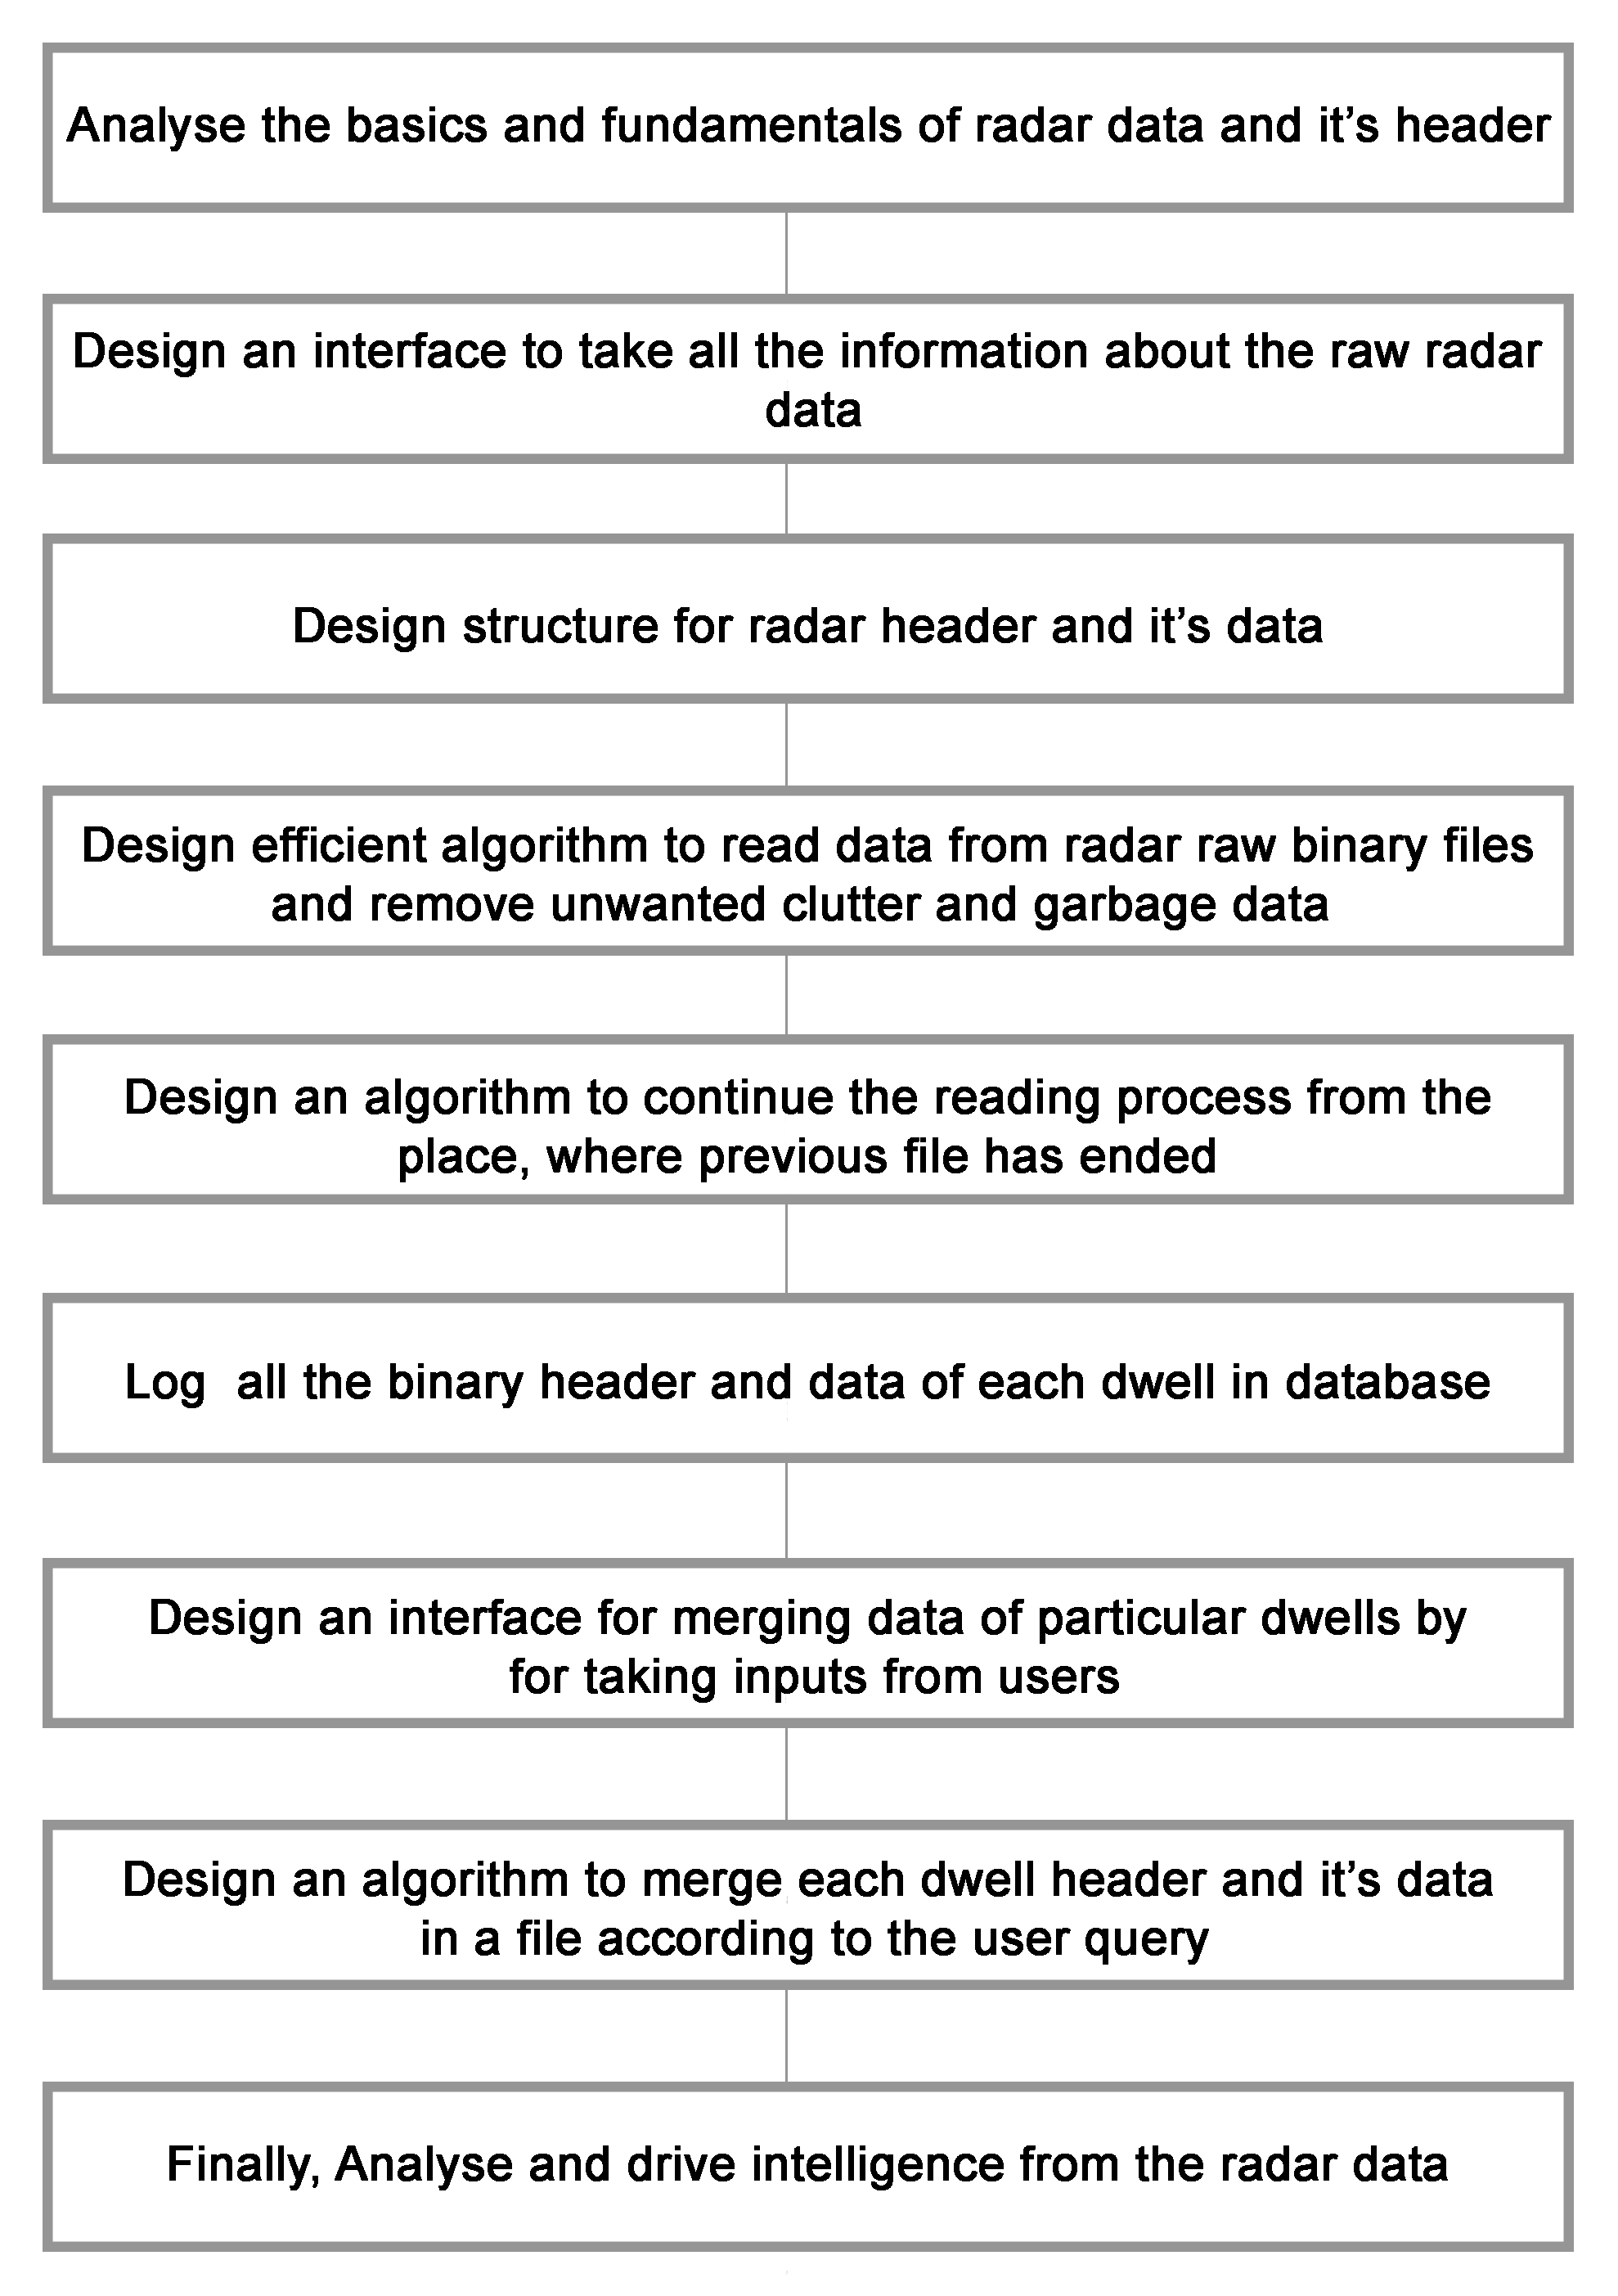
\includegraphics[width=0.8\linewidth]{steps.png}}
  \caption{Steps involved.}
  \label{fig:figure 1}
\end{figure}

\subsection{CONSTRAINTS}
Data collected from radars are voluminous. For example, a single volume of radar reflectivity data from the QRSAM, BSR radar requires about   1 GB of disk space. With a volume collected approximately every 30 minutes, this corresponds to 48 GB per day if operated for one day. Archiving and processing such large data sets every time are formidable tasks. The brute force approach of reading data every time when needed from raw files, uncompressing the data, analysing, loading another chunk, and so on, is impractical. For one, it limits access to the data and prevents parallel research activities.

\pagebreak

\title{CHAPTER 2}
\maketitle
\section{ABOUT LRDE, DRDO}

\subsection{ABOUT ORGANISATION}
\textbf{ELECTRONICS AND RADAR DEVELOPMENT ESTABLISHMENT (LRDE)} is one among the labs under \textbf{ Defence Research and Development Organization (DRDO)}. Defence Research \& Development Organisation (DRDO) works under Department of Defence Research and Development of Ministry of Defence. LRDE has its genesis in the Inspectorate of Scientific Stores created in 1939 at  Rawalpindi which was re-designated as Technical Development Establishment (Instruments and Electronics) in 1946 and located at Dehradun. In the year 1958 the Electronics Research and Development Establishment was formed at Bangalore with men and material inherited from TDE (I\&E).. 

\subsection{CORE COMPETENCIES}
\begin{itemize}
 \item	Design and Development of major sub-systems - Mechanical and Electronic Scanning Antennas, High Performance Transmitters, Exciters, Receivers, T/R Modules, Digital Signal \& Data Processors, Mechanical Engineering.
\item	Radar System Engineering for Ground based, Ship borne and Air borne systems.
\item	Environmental engineering including EMI/EMC.
\item	Radar System Integration and Evaluation
\end{itemize}
\subsection{ACTIVITIES}
Design and Development of Radar Systems are
\begin{enumerate}
\item 
\textbf{Army}
\begin{itemize}
\item	Multifunction Phased Array Radar and 3D Surveillance Radar for Akash Missile Weapon System.
\item	 Low Level 2D Radar for Fire Control and Air Defence.
\item	 Short Range Battle Field Surveillance Radar.
\item	 Weapon Locating Radar.
\item	 3D Tactical Control Radar.
	 \end{itemize}
\item
\textbf{Navy}
\begin{itemize}
\item	Maritime Patrol Radar for fixed and Rotary Wing Aircraft.
\item	Maritime Patrol Radar with SAR \& ISAR.
\item	 3D Medium Range Surveillance Radar for ASW Corvettes
\end{itemize}
\item
\textbf{Airforce}
\begin{itemize}
\item	Multifunction Phased Array Radar and 3D Surveillance Radar for Akash Missile Weapon System.
\item	Active Phased Array Radar for AEW\&C.
\item	Low level 2D radar and 3D Short \& Medium Range Surveillance Radar for Air Defence.
\item	Medium Power Radar (MPR).
\item	 Low Level Transportable Radar (LLTR).
\item	Active Electronically Scanned Array Radar (AESA).
\end{itemize}

\end{enumerate}

\pagebreak

\title{CHAPTER 3}
\maketitle
\section{ABOUT RADAR}
\subsection{RADAR FUNDAMENTALS}
Radar is acronym for Radio Detection and Ranging. Radar is an electromagnetic system for detection and location for reflecting objects. Radar can also be used to detect stationary objects buried underground. In some cases, Radar can identify as well .For example, it can identify the type of the aircrafts it has detected. It operates by radiating energy into space and detecting the eco signal reflected from an object or target. The reflected energy that is returned to the radar not only indicates the presence of a target, but by comparing received echo signal with the signal that was transmitted, its location can be determined along with other target related information. Radar can perform its functions at long or short distance and  under conditions improvises to optical and infrared sensors. Its ability to measure distance with high accuracy and weather is one of its most important attributes. The radar makes use of radio waves that are electromagnetic in nature which gets reflected when they encounter some object in their path. 
The time taken by the radio waves to go from the transmitter to the objects and in coming back to the receiver is recorded by Radar, which is used to determine the distance of objects from the Radar by the simple equation given by
 \begin{center}                                             
    R=CT/2
 \end{center}
Where R is range of the target from the Radar.
 C is speed of the electromagnetic wave which is equal to the velocity.
 T is time taken by the pulse to travel from transmitter to target and back from target to receiver.
\subsection{RADAR BLOCK DIAGRAM}
 The block diagram given below Figure 2 shows the main components of the basic radar system and their operations are:
\begin{itemize}

\item \textbf {\underline{Transmitter}:}
\\* The radar transmitter produces the short duration high-power rf pulses of energy that are into space by the antenna.
\item \textbf {\underline{Duplexer}:}
 \\*     The duplexer alternately switches the antenna between the transmitter and receiver so that only one antenna need be used. This switching is necessary because the high-power pulses of the transmitter would destroy the receiver if energy were allowed to enter the receiver.
      
\begin{figure}[H]
  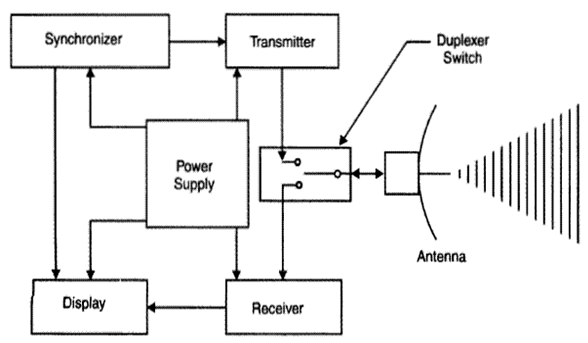
\includegraphics[width=\linewidth]{RadarBlockDiagram.png}
  \caption{Block diagram of radar.}
  \label{fig:figure 2}
\end{figure}


\item \textbf {\underline{Receive}:}
 \\*     The receivers amplify and demodulate the received RF-signals. The receiver provides video signals on the output.
\item \textbf {\underline{Radar-Antenna}:}
 \\*     The Antenna transfers the transmitter energy to signals in space with the required distribution and efficiency. This process is applied in an identical way on reception.
\item \textbf {\underline{Indicator}:}
\\* The indicator should present to the observer a continuous, easily understandable, graphic picture of the relative position of radar targets. The radar screen (in this case a PPI-scope) displays the produced from the echo signals bright blips. The longer the pulses were delayed by the runtime, the further away from the canter of this radar scope they are displayed. The direction of the deflection on this screen is that in which the antenna is currently pointing.
\end{itemize}
\subsection{RADAR FREQUENCY BANDS}
The following Table 1 shows radar frequency bands:

\begin{figure}[H]
 \centerline{\includegraphics[width=0.75\linewidth]{band.jpg}}
  \caption{Radar Frequency Bands}
  \label{fig:figure 3}
\end{figure}
 

High Frequency (HF) radars utilize the electromagnetic waves’ reflection off the ionosphere to detect targets beyond the horizon. Some examples include the United States over the Horizon Backscatter (U.S. OTH/B) radar which operates in the frequency range of, the U.S. Navy Reloadable Over The Horizon Radar (ROTHR), see Fig. 2.3-2, and the Russian Woodpecker radar. Very High Frequency (VHF) and Ultra High Frequency (UHF) bands are used for very long range Early Warning Radars (EWR). Some examples include the Ballistic Missile Early Warning System (BMEWS) search and track mono-pulse radar which operates at (Fig. 2.3-3), the Perimeter and Acquisition Radar (PAR) which is a very long range multifunction phased
array radar, and the early warning PAVE PAWS multifunction UHF phased array radar. Because of the very large wavelength and the sensitivity requirements for very long range measurements, large apertures are needed in such radar systems.


 \begin{figure}[H]
  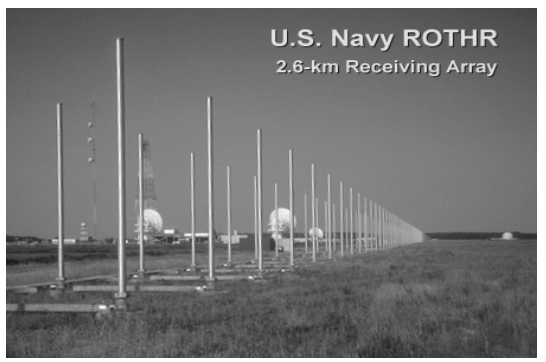
\includegraphics[width=\linewidth]{Horizonradar.png}
  \caption{U. S. Navy Over The Horizon Radar}
  \label{fig:figure 4}
\end{figure}
Radars in the L-band are primarily ground based and ship based systems that are used in long range military and air traffic control search operations. Most ground and ship based medium range radars operate in the S-band. For example, the Airport Surveillance Radar (ASR) used for air traffic control, and the ship based U.S. Navy AEGIS (Fig. 2.6-4) multifunction phased array are S-band radars. The Airborne Warning And Control System (AWACS) shown in Fig. 2.6-5 and the National Weather Service Next Generation Doppler Weather Radar (NEXRAD) are also S-band radars. However, most weather detection radar systems are C-band radars. Medium range search and fire control military radars and metric instrumentation radars are also C-band.


 \begin{figure}[H]
  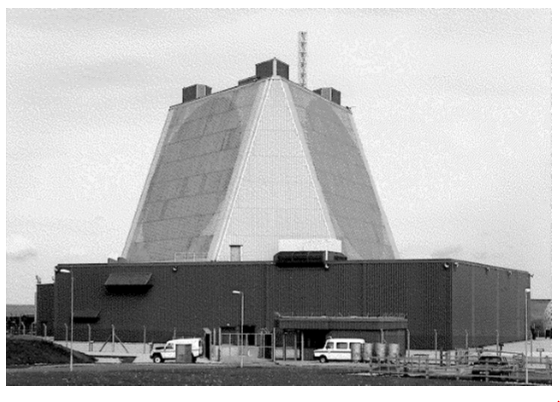
\includegraphics[width=\linewidth]{fylingdales.png}
  \caption{Fylingdales BMEWS - United Kingdom}
  \label{fig:figure 5}
\end{figure}


\begin{figure}[H]
  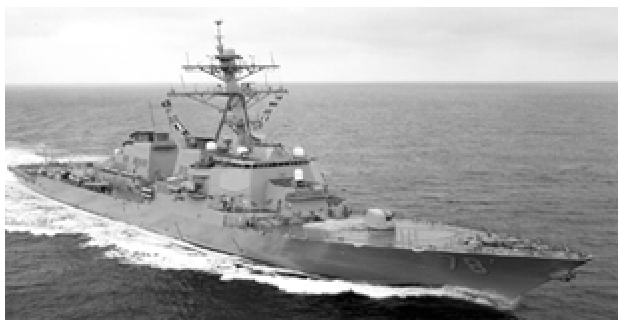
\includegraphics[width=\linewidth]{Navy.png}
  \caption{U. S. Navy AEGIS}
  \label{fig:figure 6}
\end{figure}



 \begin{figure}[H]
  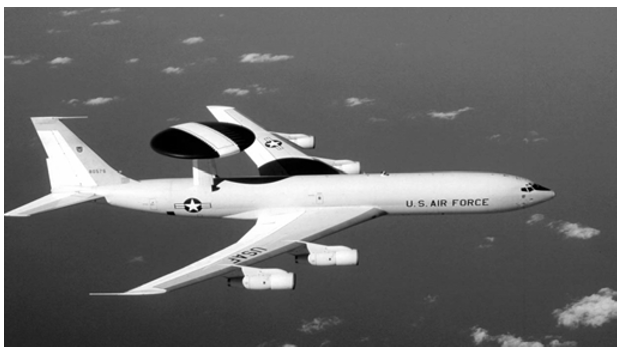
\includegraphics[width=\linewidth]{airforce.png}
  \caption{ U. S. Air Force AWACS}
  \label{fig:figure 7}
\end{figure}

The X-band is used for radar systems where the size of the antenna constitutes a physical limitation; this includes most military multimode airborne radars. Radar systems that require fine target detection capabilities and yet cannot tolerate the atmospheric attenuation of higher frequency bands may also be X-band. The higher frequency bands (Ku, K, and Ka) suffer severe weather and atmospheric attenuation. Therefore, radars utilizing these frequency bands are limited to short range applications, such as the police traffic radars, short range terrain avoidance, and terrain following radars. Milli-Meter Wave (MMW) radars are mainly limited to very short range Radio Frequency (RF) seekers and experimental radar systems.
\subsection{RANGE PERFORMANCE OF RADARS}
The maximum range R\textsubscript{max} equation for radars are:
\[R_{max} = \dfrac{P_tGA_e\sigma}{4\pi^{2}S_{min}} \]

where, \\ \indent P\textsubscript{t} = Transmitted power, in watts,
              \\ \indent G = Antenna gain,
              \\ \indent A\textsubscript{e} = Antenna effective aperture, in m\textsuperscript{2}
                         \\ \indent $\sigma$ =  Radar cross-section of the target, in m\textsuperscript{2}
              \\ \indent S\textsubscript{min} =  Minimum detectable signal, in watts\\


All the above parameters, except $\sigma$  , are to some extent under the control of the radar designer.
\\ In practice, the simple radar equation does not predict the range performance of actual radar equipment’s to a satisfactory degree of accuracy.
 In many cases the actual range might be half of that predicted by the above equation. Some of the major reasons for this are the following:
\begin{itemize} 
\item  Failure of the equation to explicitly include various losses that can occur throughout the system.
\item Loss of performance usually experienced when electronic equipment are operated in the field, as against when they are operated under laboratory conditions.
\item Statistical and unpredictable nature of the various parameters in the radar equation.
\end{itemize}
Both S\textsubscript{min} and $\sigma$ are statistical in nature and must be expressed as such in statistical terms. other statistical factors which affect radar performance are meteorological conditions along the propagation path and performance of the radar operator, if one is employed.
In view of the above, specification of radar range is usually given as the probability that the radar will detect a certain type of target at a particular range.

\subsection{HISTORY OF RADAR}
 Neither a single nation nor a single person can say that the discovery and development of radar technology was his (or its) own invention. One must see the knowledge about “Radar” than an accumulation of many developments and improvements, in which any scientists from several nations took part in parallel. In the past, there are nevertheless some milestones, with the discovery of important basic knowledge and important inventions:
 
\begin{itemize}
\item \textbf {1865  :} The Scottish physicist James Clerk Maxwell presents his “Theory of the Electromagnetic Field” (description of the electromagnetic waves and their propagation) He demonstrated that electric and magnetic fields travel through space in the form of waves, and at the constant speed of light.

\item \textbf {1886 : }The German physicist Heinrich Rudolf Hertz  discovered electromagnetic waves, thus demonstrating the Maxwell theory.

\item \textbf { 1897 :  }The Italian inventor Guglielmo Marconi achieved the first long distance transmission of electromagnetic waves. In his first experiments he used a wire to a wooden pole. In Italian a tent pole is known as lantenna centrale, and the pole with a wire alongside it used as an aerial was simply called lantenna. Today Marconi is known as pioneer of radio communication.

\item \textbf {1900 :  }Nicola Tesla suggested that the reflection of electromagnetic waves could be used for detecting of moving metallic objects.

\item \textbf {1904 :  }The German engineer Christian Hulsmeyer invents the "telemobiloscope" for a traffic monitoring on the water in poor visibility. This is the first practical radar test. Hülsmeyer apply his invention for a patent in Germany, France and the United Kingdom.

\item \textbf {1921 :  }The invention of the Magnetron as an efficient transmitting tube by the US-American physicist Albert Wallace Hull.

\item \textbf {1922 : }The American electrical engineers Albert H. Taylor and Leo C. Young of the Naval Research Laboratory (USA) locate a wooden ship for the first time.

\item \textbf {1930 :  }Lawrence A. Hyland (also of the Naval Research Laboratory), locates an aircraft for the first time.

\item \textbf {1931 : }In Britain the first known proposal for a radar system came from William A. S. Butement and P. E. Pollard in January 1931. They equipped a ship with radar. As antennae were used parabolic dishes with horn radiator. Although their equipment produced short-range results the work was abandoned for lack of government support.

\item \textbf {1933 : }On the basis of the in 1931 from himself invented sonar, Rudolph Kühnhold presented a so called “Funkmessgerat”. It worked on a wavelength of 48 cm and the transmitter had a power of about 40 Watts. From these tests, the Freya-radar was developed, which was produced in series beginning in 1938.

\item \textbf {1935 : } Robert Watson-Watt (later: Sir Robert) suggested that radio waves might be used to detect aircraft at a distance and outlined a means of doing so. Intensive research began and by 1939 Britain possessed a defensive chain of highly secret Radio Direction Finding (RDF) stations.

\item \textbf {1936 :} The development of the Klystron by the technicians George F. Metcalf and William C. Hahn, both General Electric. This will be an important component in radar units as an amplifier or an oscillator tube.

\item \textbf {1939 : }Two engineers from the university in Birmingham, John Turton Randall und Henry Albert Howard Boot built a small but powerful radar using a Multicavity-Magnetron. The B–17 airplanes were fitted with this radar. Now they could find and thus combat the German submarines in the night and in fog.

\item \textbf {1940 :} Different radar equipment’s are developed in the USA, Russia, Germany, France and Japan
.
Driven by general war events and the development of the Air Force to major branch of service, the radar technology undergoes a strong development boost during the World War II, and radar sets were used during the "Cold War" in large numbers along the inner German border.
\end{itemize}

\subsection{ TYPES OF RADAR}
The types of radar are classified into four categories:
\begin{enumerate}
\item	Frequency 
\item	Waveform 
\item	PRF Pulse 
\item	Application
\end{enumerate}

 \begin{figure}[H]
  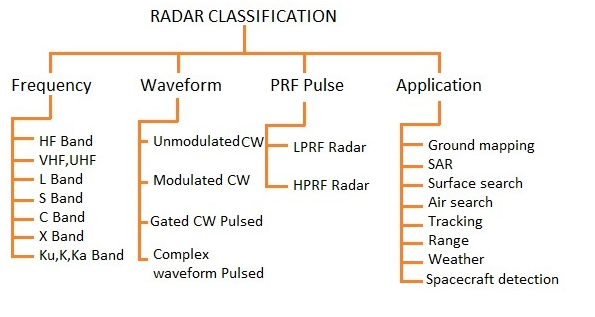
\includegraphics[width=\linewidth]{radartypes.png}
  \caption{ Types of Radar}
  \label{fig:figure 8}
\end{figure}
\subsubsection{Frequency based radar types}
 Following are the radar types based on frequency bands:
 \begin{enumerate}
\item	HF Band Radars
\item	VHF and UHF band radars
\item	L-Band Radars
\item	S-Band Radars 
\item	C-Band Radars 
\item	X-Band Radars 
\item	Ku, K, Ka Band Radars 
\item	Infrared, Visible light band radars
\end{enumerate}

\subsubsection{Waveform Based radar classification}
 Following are the radar types based on waveform:
\begin{enumerate}
\item	Unmodulated CW radar
\item	Modulated CW radar
\item	Gated CW pulsed radar
\item	Complex waveform pulsed radars
\end{enumerate}

\subsubsection{PRF Based radar classification}
Following are the radar types based on PRF:
\begin{enumerate}
\item	LPRF (Low Pulse Repetition Frequency) Radar.
\item	HPRF (High Pulse Repetition Frequency) Radar.
\end{enumerate}

\subsubsection{Application based radar classification}
 Following are the radar types based on their applications of use: 
\begin{enumerate}
\item	Search radars (surface, air)
\item	Warning radars such as weather forecast radars 
\item	Spacecraft detection radars
\item	Fire control radars
\item	Ground mapping radars
\item	SAR 
\item	Air to Surface radars 
\item	Sea surface radar 
\item	Ground moving target search radars 
\item	 Tracking radar
\item	 Range radar
\item	 velocity search radar
\end{enumerate}

\subsection{APPLICATIONS OF RADAR}
Detection and search radar includes the “early warning radar”, used for long-range detection of objects, and the target acquisition(AT), used to locate surface-to-air missiles(SAM).These types are frequently used in the military and in coastal surveillance, as well as for detecting car speed during highway patrol.
Missile guidance system are used to locate the target of a missile. This is often present in military aircraft.
Radar for biological research includes tracking birds and insects to trace their migration patterns. Bird radar is also being used at NASA’s Kennedy space center in Florida to track the presence of birds, especially vultures, near launching pads. Trap and release programs have been implemented to prevent birds accidently impacting the shuttles after lift off.
Air traffic control and navigation radar is used by airports to ensure the safety of planes. This type detects the proximity of an aircraft and identifies the identity and altitude of the plane. Radio beacons and distance measuring equipment(DME) also fall into category.
Weather-sensing radar systems are mostly used to measure and locate precipitation. They can also measure wind direction and speed. 
         Other applications of radar are:
 \begin{enumerate}
\item \textbf {On ground :} Detection, location, and tracking of aircraft and space targets.

\item \textbf {In the air :} Detection of other aircraft, ships, or land vehicles; mapping of land; storm avoidance, terrain avoidance, and navigation.

\item \textbf {On the sea :} Navigation aid and safety device to locate buoys, shore lines, other ships, and for observation of aircraft.

\item \textbf {In space :} Guidance of spacecraft; remote sensing of land and sea.
\newline
\\ \textbf{Some specific applications are as follows:}

\item \textbf {Air traffic control :} Controlling of air traffic in the vicinity of airports; and also for automated landing.

\item \textbf {Aircraft navigation :} Weather avoidance to indicate regions of severe precipitation; terrain following/terrain avoidance (TF/TA); radio altimeter and doppler navigator are also radars.

\item \textbf {Ship safety :} Collision avoidance; detection of navigation buoys.

\item \textbf {Space :} Rendezvous and docking; landing on the moon and other planets; detection and tracking of satellites.

\item \textbf {Remote sensing :} Sensing of geophysical object, or the ”environment” like weather, cloud cover, earth resources, water resources, agriculture, forests, geological formation, etc. This is usually done from aircraft or satellites.

\item \textbf {Law enforcement :} To monitor speed of vehicles in traffic.

\item \textbf {Military :} Surveillance and navigation; control and guidance of weapons. The largest use of radars occurs here.

\end{enumerate}

\subsection{RADAR SUBSYSTEMS}
The following figure 6.3 shows the Product tree of MFR: 

 \begin{figure}[H]
  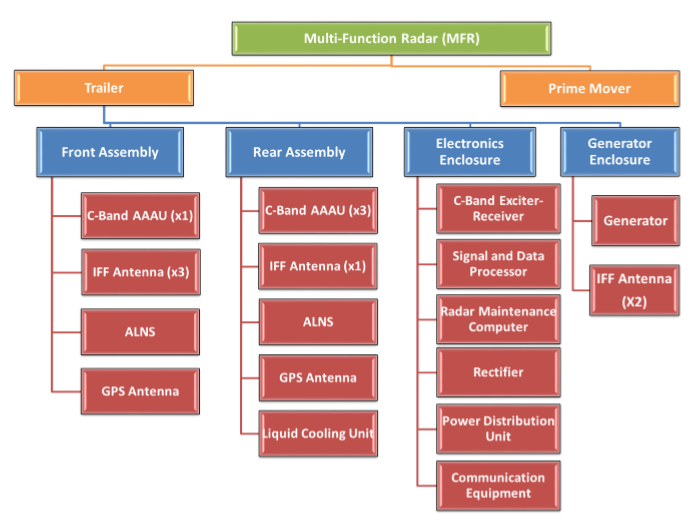
\includegraphics[width=\linewidth]{MFR.png}
  \caption{Product tree of MFR}
  \label{fig:figure 9}
\end{figure}
 \begin{enumerate}
\item \textbf {C-Band Active Array Antenna Unit (AAAU)}
\\The Active Array Antenna Unit (AAAU) consists of the radiating elements array, the Transmit/Receive Modules (TRMs), the power combiner network, the control signal distribution network and the beam steering network. This unit radiates energy in to the coverage volume of interest and collects the echo signals from the environment.
\item \textbf {C-band Exciter-Receiver}  
\\*	This unit consists of the exciter that generates the required RF and timing signals and the receiver which down converts the received echoes.

\item \textbf {Signal and processor}
\\ This unit processes the received signals for Detection, Clutter suppression and parameter extraction are performed by this unit.

\item \textbf {Radar computer}
\\	This subsystem is the brain of the radar and consists of a radar controller, radar data processor, embedded simulator and the interfaces to the external systems. 

\item \textbf {Commander’s console}
\\	The commander’s console consists of a workstation and a display screen and functions as the interface between the operator / commander and the radar.

\item \textbf {Power system}
\\	This consists of a diesel generator, rectifiers and power distribution unit.

\item \textbf {Liquid cooling unit}
\\	This subsystem is responsible for removing heat generated in other subsystems. It consists of a compressor, a pump to circulate a coolant and a heat exchanger.

\item \textbf {Prime Mover with Trailer}
\\	The entire radar system is mounted on this vehicle. The pallet of this vehicle will have a support structure mounted on it which supports all other subsystems.

\item \textbf {Inertial Navigation Unit (INU)}
\\	This subsystem provides the attitudes of the MFR platform.

\item \textbf {IFF unit}
\\	The IFF unit consists of 4 IFF antennas and the IFF interrogator.

\item \textbf {Communication system}
\\       The MFR consists of communication equipment, radio sets and voice communication handsets. MFR will interface with all data communication equipment via gigabit Ethernet. The communication equipment will interact with the external systems via wireless link, with wired link as backup.
	
\item \textbf {AC-DC Rectifier}
\\     The Rectifier receives 415V AC (L-L), 50 Hz, 3Ø power from Diesel Generator (DG) as input and converts it to 320V DC and supplies it to different subsystems.

\end{enumerate}
\pagebreak

\title{CHAPTER 4}
\maketitle
\section{ABOUT DATABASES}
\subsection{INTRODUCTION}
A database management system (DBMS) is a software package with computer programs that control the creation, maintenance, and use of a database. It allows organizations to conveniently develop databases for various applications by database administrators (DBAs) and other specialists. A database is an integrated collection of data records, files, and other objects. A DBMS allows different user application programs to concurrently access the same database. DBMSs may use a variety of database models, such as the relational model or object model, to conveniently describe and support applications. It typically supports query languages which are in fact high-level programming languages, dedicated database languages that considerably simplify writing database Application programs.  A DBMS provides facilities for controlling data access, enforcing data integrity, managing concurrency control, and recovering the database after failures and restoring it from backup files, as well as maintaining database security.
\\
\\ \textbf{Definition:}
\\A database management system (DBMS) is the software that allows a computer to perform database functions of storing, retrieving, adding, deleting, and modifying data. Relational database management system (RDBMS) implements the relational model of tables and relationships.
\\
\\ \textbf{Examples:}
\\Microsoft access, MySQL, Microsoft SQL server, oracle and File maker pro are all examples of database management systems.
\\
\\ \textbf{Types of database management system}
  \\Different types of DBMS are as follow:
 \begin{itemize}
\item	Hierarchical DBMS  
\item	Network DBMS
\item	Relational DBMS
\item	Flat file DBMS
\item	 Object Oriented DBMS        
\end{itemize}


\subsubsection{\textbf{Hierarchical DBMS:}}                                
 \begin{figure}[H]
 
  \centerline{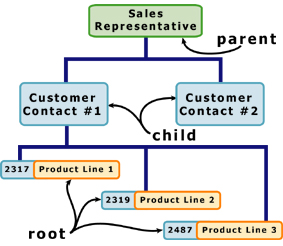
\includegraphics[width=0.7\linewidth]{hierarchical.jpg}}
  \caption{Hierarchical DBMS}
  \label{fig:figure 10}
\end{figure}
One of the earliest database management systems was based on the Hierarchical model. Here data can be organized in the form of free structure or level-by-level manner with one limitation that is "every sub node or child node should have only one parent node".

\subsubsection{\textbf{Network DBMS: }}
    Network databases are similar to hierarchical databases by also having a hierarchical structure. There are a few key differences, however. Instead of looking like an upside-down tree, a network database looks more like a cobweb or interconnected network of records. In network databases, children are called members and parents are called owners. The most important difference is that each child or member can have more than one parent (or owner). 
Like hierarchical databases, network databases are principally used on mainframe computers. Since more connections can be made between different types of data, network databases are considered more flexible. However, two limitations must be considered when using this kind of database.
\newpage
\subsubsection{\textbf{Relational DBMS:}}
 \begin{figure}[H]
    \centerline{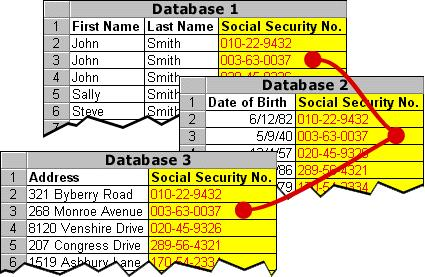
\includegraphics[width=0.65\linewidth]{relational.jpg}}
  \caption{Relational DBMS:}
  \label{fig:figure 11}
\end{figure}
RDBMS are most important database system used in the software industry today. It was exclusively used to establish the relation the relationship between two-database objects. One of the database objects is one table.
\\The Relationship may be
\begin{itemize}
\item One - One 
\item One - Many
\item Many - One
\item Many – Many
\end{itemize}
\subsubsection{\textbf{Flat files DBMS:}}
 In flat file database management system the user specifies the data attributes for one table at a time, storing data independently from application.
\subsubsection{\textbf{Object Oriented DBMS:}}
 \begin{figure}[H]
    \centerline{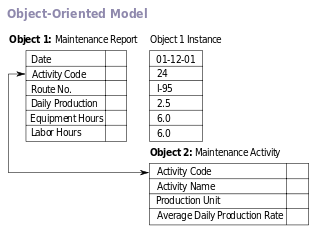
\includegraphics[width=0.65\linewidth]{object.png}}
  \caption{Object Oriented DBMS:}
  \label{fig:figure 12}
\end{figure}
Object Oriented DBMS Database that stores data elements as objects. Uses of object-oriented concepts. The term object oriented is abbreviated by OO or O-O
An object database (also object-oriented database management system) is a database management system 
In which information is represented in the form of objects as used in object-oriented programming. Object databases are different from relational databases and belongs together to the broader database management system.
Object databases have been considered since the early 1980s and 1990s; they may be slower in simple mass commercial data transaction. Object databases main usage is in object oriented areas. 
      
                           
\subsection{ADVANTAGES OF DBMS:} 
There are many advantage of database management system; some of them are as follows.
 \begin{itemize}
\item[]\textbf{Warehouse of Information:}
The database management systems are warehouses of information, where large amount of data can be stored. The common examples in commercial applications are inventory data, personnel data . The best examples for the same would be the address book of a Cell phone, digital diaries, etc. 
\item[]\textbf{Defining Attributes:} 
The unique data field in a table is assigned a primary key. The primary key helps in the identification of data. It also checks for duplicates within the same table, thereby reducing data redundancy. There are tables, which have a secondary key in addition to the primary key. The secondary key refers to the primary key of another table, thus establishing a relationship between the two tables. 
\item[]\textbf{Systematic Storage:} 
The data is stored in the form of tables. The tables consist of rows and columns.
\item[]\textbf{Changes to Schema:} 
The table schema can be changed and it is not platform dependent. Therefore, the tables in the system can be edited to add new columns and rows without hampering the applications that depend on that particular database.
\item[]\textbf{No Language Dependence:} 
The database management systems are not language dependent. Therefore, they can be used with various languages and on various platforms. 
\item[]\textbf{Table joins:} 
The data in two or more tables can be integrated into a single table. This enables to reduce the size of the database and helps in easy retrieval of data.
\item[]\textbf{Multiple Simultaneous Usages:} 
            The database can be used simultaneously by a number of users. 
\item[]\textbf{Data Security:}
 Database management systems help to keep the data secured.
 \item[]\textbf{Data Consistency:} 
            Data consistency ensures a consistent view of data to every user. It includes the accuracy,validity and integrity of related data. 
  \end{itemize}          
 \subsection{DISADVANTAGES OF  DBMS}
Some disadvantages of DBMS are as follow:
\begin{itemize}
\item A complex conceptual design process;
\item	The need to hire database-related employees;
\item	High DBMS acquisition costs;
\item	A more complex programmer environment;
\item	Potentially catastrophic program failures;
\item	A longer running time for individual applications; 
\item	Database systems are complex, difficult, and time-consuming to design
\item	Substantial hardware and software start-up costs
\item	Damage to database affects virtually all applications programs
\item	Initial training required for all programmers and users.
\end{itemize}
\textbf{Example of database management system}
\begin{enumerate}
\item	SQL
\item	ORACLE
\item	FOXPRO
\item	MS ACCESS
\item	MY SQL
\end{enumerate}

\pagebreak

\title{CHAPTER 5}
\maketitle
\section{ABOUT QRSAM}
\subsection{QUICK REACTION SURFACE-TO-AIR MISSILE (QRSAM)}
Quick Reaction Surface ­to­ Air Missile (QRSAM) the homegrown canister ­based sophisticated high speed missile capable of destroying aerial targets and short range missiles.
 \begin{figure}[H]
    \centerline{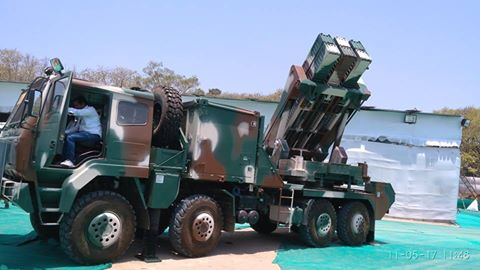
\includegraphics[width=\linewidth]{qrsam.jpg}}
  \caption{QRSAM launching High Mobility Vehicle (HMV)}
  \label{fig:figure 13}
\end{figure}
\subsubsection{Features:}
\begin{itemize}
\item[] Canister mounted QRSAM is a highly mobile air defence system which comes with 100 percent kill probability, and has the capability to neutralise aerial targets like fighter jets, cruise missiles and air ­to ­surface missiles as well as short-range ballistic missiles. QRSAM is also a vital component in India’s \textbf{“Cold Start”} Doctrine which will ensure the safety of forward Army formations in Enemy territories.
\item[] QRSAM and Man-portable air-defense systems (MANPADS) are only surface-to-air missile systems that are capable and also is highly mobile to move with strike corps deep into Pakistani territory to destroy selected targets.
\item[] QRSAM Air Defence System has a Surveillance and target tracking systems, Command and Control Systems, Missile launchers which can provide Air Defence coverage while on the move. 
\item[] Missiles have a reaction time of fewer than 6 Seconds once launch command of the missile is issued to the missile launcher. The missile system can engage multiple targets within a range from 3 km to 30 km in azimuth and 30 m to 6 km in altitude.
\item[] The missile can engage aircraft at 500m/s at 20 km and 300m/s at 30 km, along with helicopters and UAVs. The missile also has terminal guidance using an RF seeker. The system has AESA radar with X-band Quad Transmit Reciever Modules (QTMs), Two Way Data Link (TWDL) and IFF. the \textbf{Battery Surveillance Radar (BSR)} has a range up to 120 km and the\textbf{ Multi-Function Fire Control Radar (BMFR)} has a tracking range of up to 80 km. 
\item[] Truck based QRSAM Air Defence System can move at speed of 50kmph and has the ability to operate nearly 8 hours at a stretch without the need for refuelling. \textbf{High Mobility Vehicle (HMV)} used are capable of being operated in plains, deserts,semi-deserts, terrains found in India and can also be transported through broad gauge rakes of Indian railways. HMV also has NBC (nuclear, biological, chemical) system installed which ensures reliable protection of the crew and internal equipment against mass destruction weapons. HMV also have a Navigation system and Night vision devices to help Driver and Commander to move in the dark and also in unfamiliar terrains.
\item[] QRSAM Air Defence System unlike Stationary Mobile Air Defence System like Akash and MR-SAM Surface to Air Missiles have fine tuned Surveillance and target tracking systems which have a higher density of aerial scans to reduce their detection time and improve their reaction time while operating in Enemy Territories and the missile can also be fired without missile launcher HMV being stopped. QRSAM Air Defence System is a critical component in India’s \textbf{“Cold Start”} Doctrine which has the ability not only to stop Aerial attacks from rival Air Force but also to neutralise Pakistan’s Solid fueled nuclear-capable tactical ballistic missile system Nasr (Hatf IX) which was specifically developed to attack “mechanized forces like armed brigades and divisions.
\end{itemize}
\subsubsection{Radar System of QRSAM}
\begin{itemize}
\item QRSAM system provides mobile area air defense missile cover to the mechanized assets of the Army. The radar unit in a QRSAM battery consists of one \textbf{Battery Surveillance Radar (BSR)} and \textbf{4 Battery Multi Function Radar (BMFR)}
 \begin{figure}[H]
    \centerline{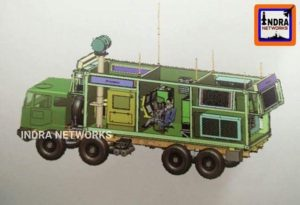
\includegraphics[width=0.7\linewidth]{qrsam-radar.jpg}}
  \caption{QRSAM Radar on High Mobility Vehicle (HMV)}
  \label{fig:figure 14}
\end{figure}
\item The BSR and BMFR ue state of the art active phased array technology combined with advanced signal processing and data processing algorithms to detect and track fixed wing aircrafts including hovering helicopters in intense EW environment.
\pagebreak
\begin{table}
\centerline {\begin{tabular}{p{0.2\textwidth}p{0.2\textwidth}p{0.2\textwidth}} \\ \toprule
&\textbf{BSR} & \textbf{BFSR}\\ \midrule
\textbf{Frequency Band} & C-band & X-band \\ \midrule
\textbf{Range} & 120km for 2m\textsuperscript{2} & 80km for 2m\textsuperscript{2} \\ \midrule
\textbf{Angular Coverage} & Az : 360$^{\circ}$ & Az : 360$^{\circ}$   \\ 
& El : 0 to 60$^{\circ}$ &  El : 0 to 60$^{\circ}$\\ \midrule
\textbf{Target Altitude} & 30m - 6km & 30m - 6km\\ \midrule
\textbf{Antenna Size} & 1.5m X 1m & 0.9m x 0.9m\\ \midrule
\textbf{Resolution} & Range : 30m& Range : 30m\\ \midrule
&Az   : 3$^{\circ}$ & Az    : $^{\circ}$\\
&El     : 4$^{\circ}$ & El     : 3$^{\circ}$\\ \midrule
\textbf{Accurac}y & Range : 30m & Range : 30m\\ 
&Az     : 8 mrad & Az      : 5 mrad\\
&El       : 8 mrad & El       : 5 mrad\\  \midrule
\textbf{Max Target Speed} & 700 m/s & 700 m/s\\ \bottomrule
\end{tabular}}
\caption{Specification of QRSAM Radar}
\end{table}

\item The BSR and BMFR use advanced platform motion compensation and electronic stabilization algorithms along with high accuracy motion sensors. Both radars are mounted on 8x8 High Mobility Vehicles and are capable of operating on the move in plains, deserts and semi-deserts.
\end{itemize}

\pagebreak

\title{CHAPTER 7}
\maketitle
\section{RESULT OBTAINED}
\subsection{Output Results}

\subsubsection{PSP Logger}
 \begin{figure}[H]
    \centerline{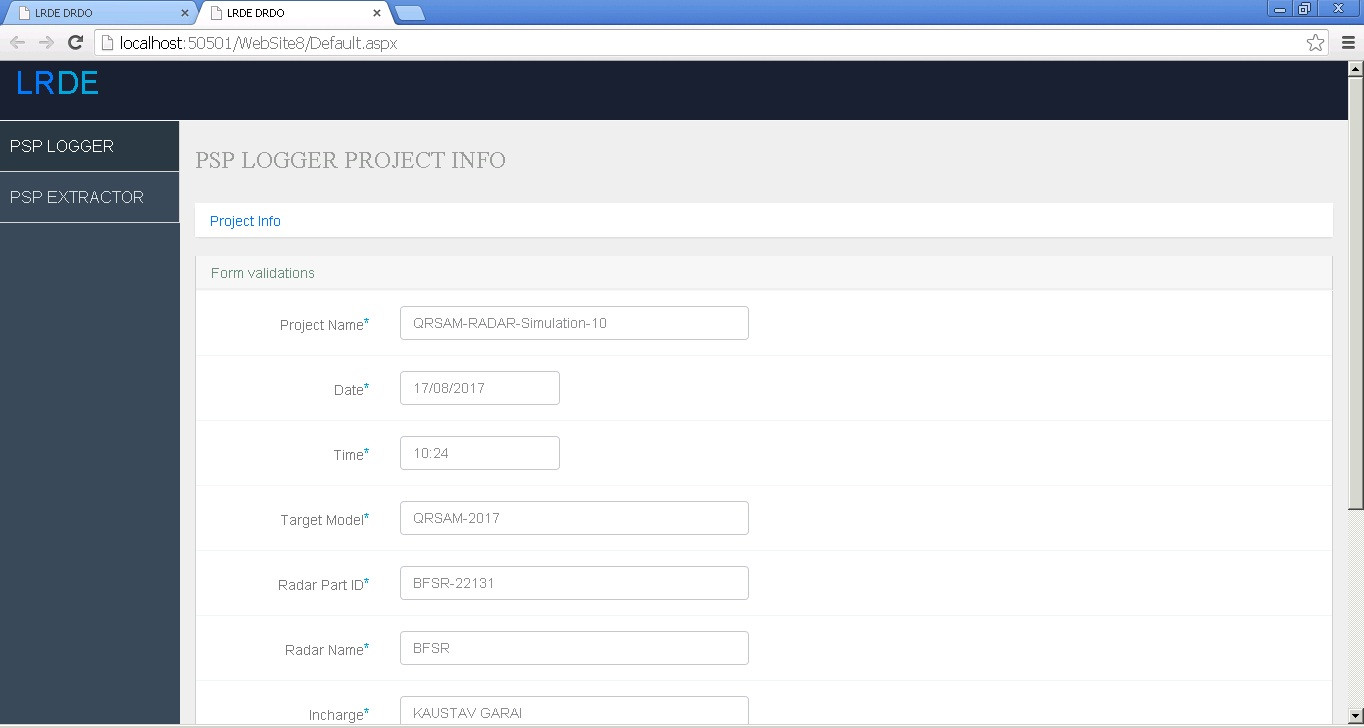
\includegraphics[width=\linewidth]{LoggerFrontPage.jpg}}
  \caption{Web Application : PSP Logger Front Graphical User Interface}
  \label{fig:figure 15}
\end{figure}
 The Figure 15 shows the Graphical User Interface(GUI) of PSP logger which takes all the information of the project 
  The input field includes :
  \begin{itemize} 
  \item[] \textbf{Project Name : }Which describes the name of the project from which the raw data has been produced.
  \item[] \textbf{Date : }Date on which the radar data was collected. 
  \item[] \textbf{Time : }Time when the data was collected.
  \item[] \textbf{Target Model : }Target model of the radar whose data is to be logged.  
  \item[] \textbf{Radar Part ID : }Model of radar whose data is to be logged.
  \item[] \textbf{Radar Name : }Name of the radar.
  \item[] \textbf{Incharge : }Name of project incharge.
  \item[] \textbf{Location : }Location where the testing of radar is done.
  \item[] \textbf{Comment : }Other information about the project.
  \end{itemize}
  When the user clicks submit button after filling all the inputs, the user is redirected to page as show in Figure 16 which contains one field.\\
   \begin{figure}[H]
    \centerline{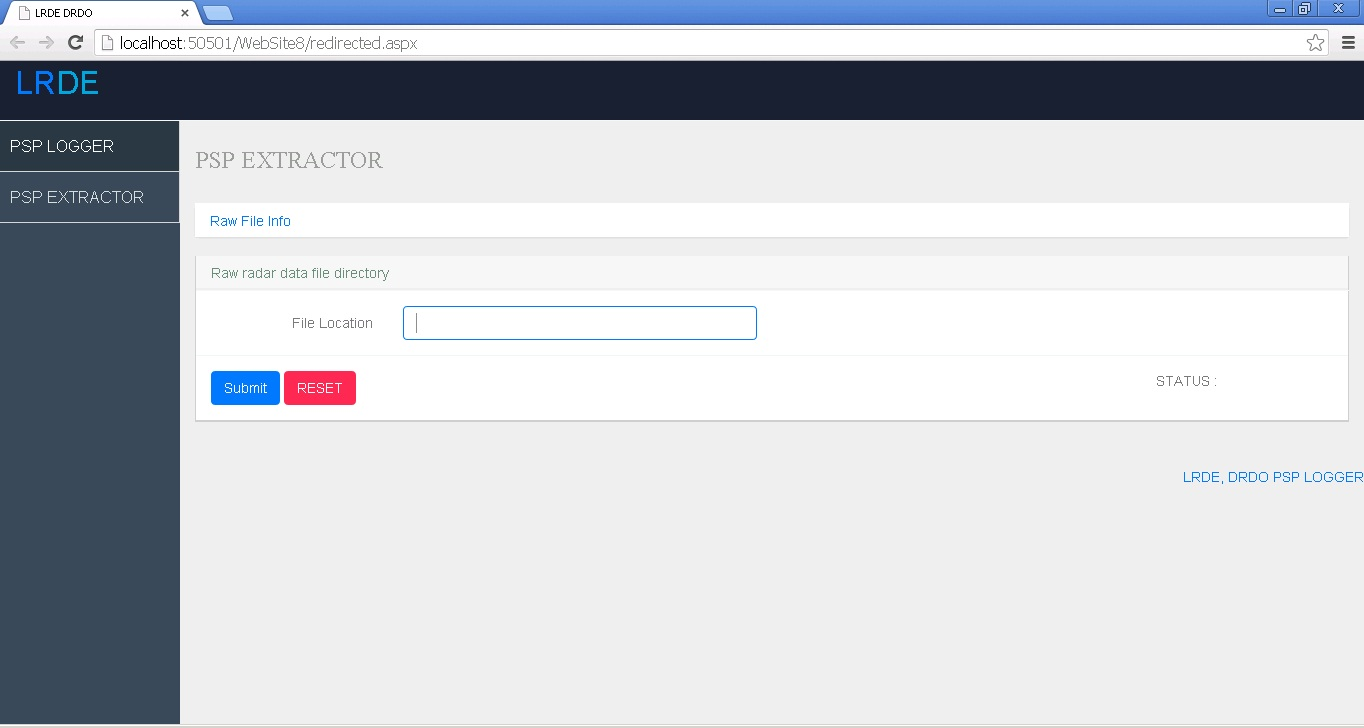
\includegraphics[width=\linewidth]{DirectoryPage.jpg}}
  \caption{Web Application : PSP logger file directory page}
  \label{fig:figure 17}
\end{figure}  
  
\indent \textbf{File Directory :} It takes the path of the raw radar binary files which is to \indent be processed and logged.\\
\\When the user clicks submit button all the files are read one by one and data is automatically stored in a database table named dwelldata and Project.

 \begin{figure}[H]
    \centerline{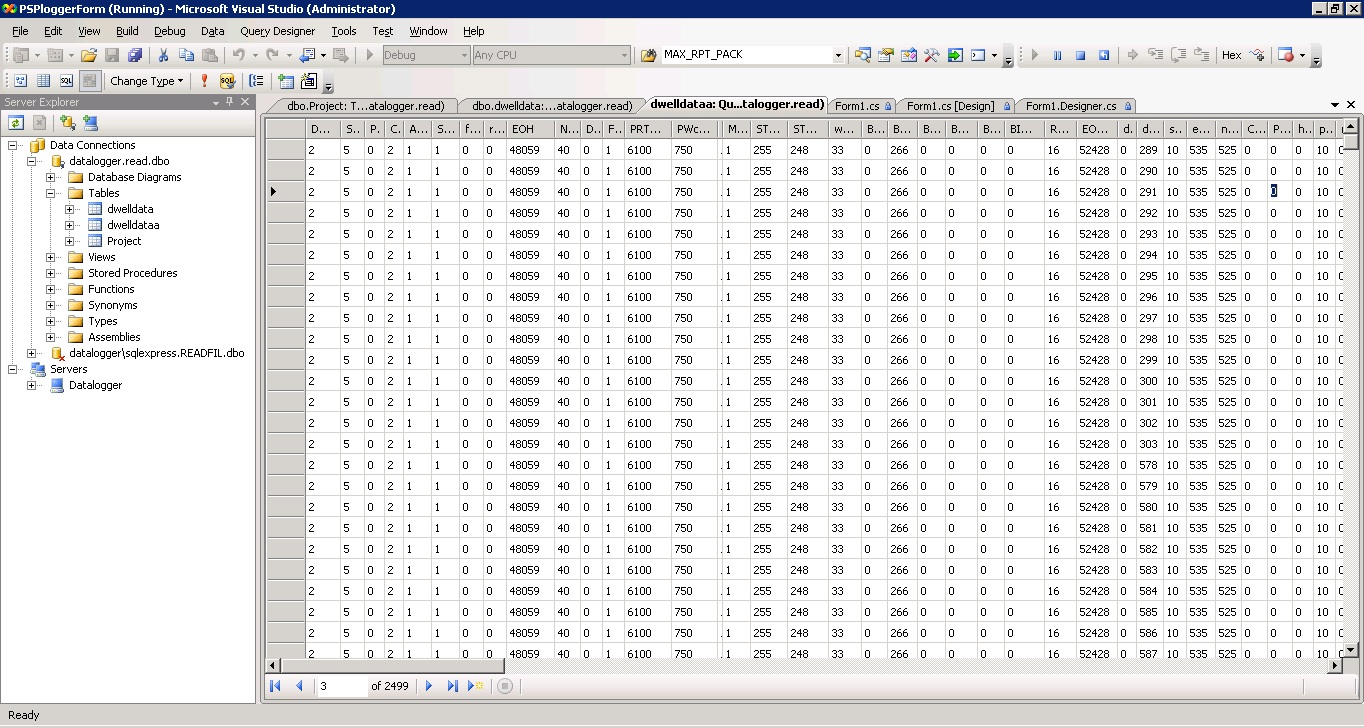
\includegraphics[width=\linewidth]{database_table_data2.jpg}}
  \caption{Database : Table - dwelldata with various fields which contains all the header and data of radar after processing, it also saves the clean binary header+data of particular dwells in a varbinary column of table which will be used in PSP merger }
  \label{fig:figure 18}
\end{figure}  
  
   \begin{figure}[H]
    \centerline{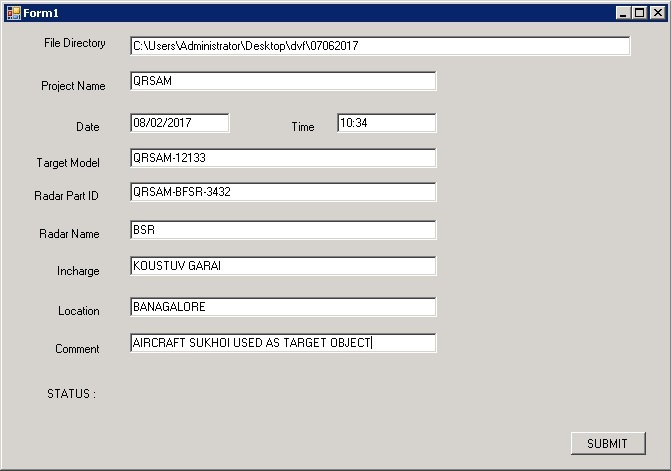
\includegraphics[width=0.8\linewidth]{PSPloggerform.jpg}}
  \caption{Windows form version of PSP Logger}
  \label{fig:figure 19}
\end{figure}  

 \begin{tcolorbox}[title = NOTE]
The STATUS label in the application provides information about the process thread, it tells whether the process has started, is in execution or it has completed. The application also show messagebox in both types of PSP Logger application to describe the status of process thread.
 \end{tcolorbox}
  \subsubsection{PSP Merger}
    \begin{figure}[H]
  \centerline{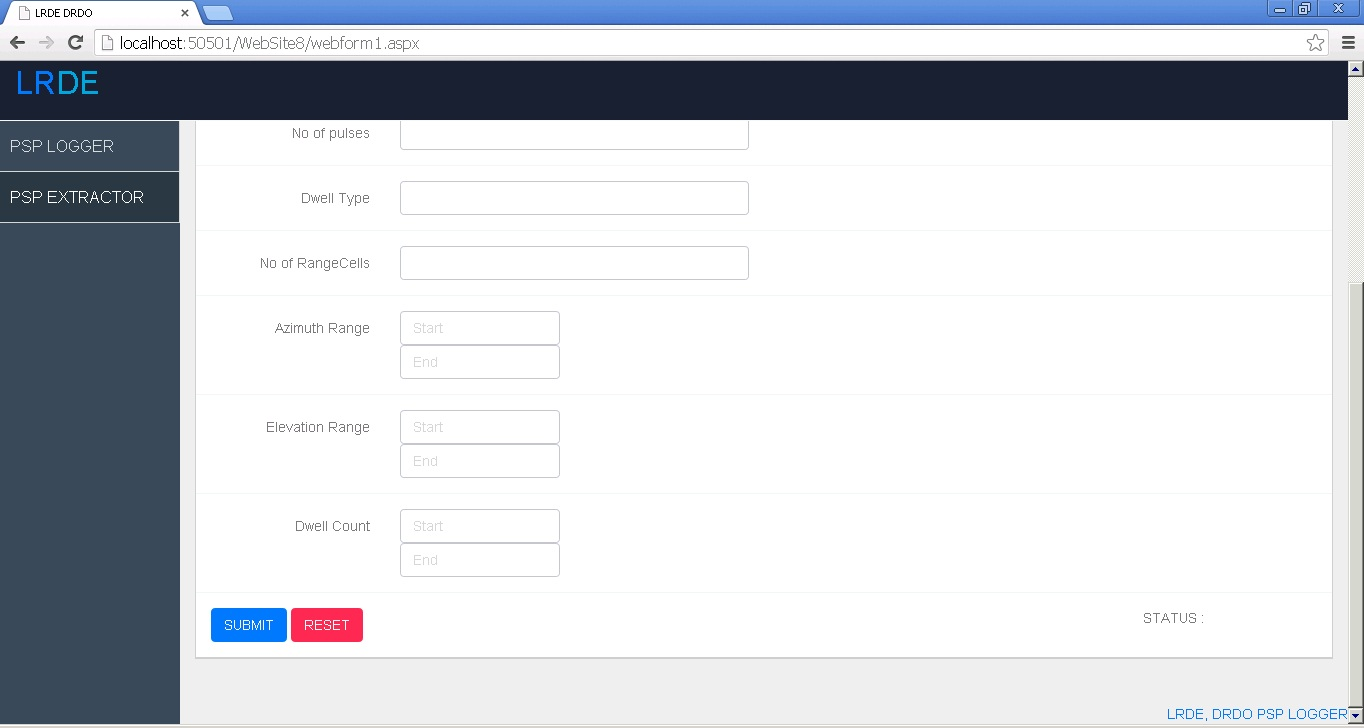
\includegraphics[width=\linewidth]{extractor2.jpg}}
  \caption{Web Appliction : PSP Merger Graphical User Interface}
  \label{fig:figure 20}
\end{figure}  
 \begin{figure}[H]
  \centerline{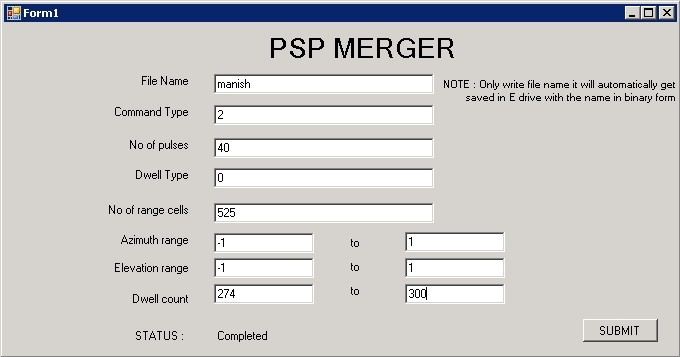
\includegraphics[width=\linewidth]{PSPmerger.jpg}}
  \caption{Windows form version of PSP Logger}
  \label{fig:figure 21}
  \end{figure}
 The Figure 20 shows the Graphical User Interface(GUI) of PSP Merger which takes all the information of the radar header fields and produce a merged binary files accourding to the inputs  in binary format. It produces files free from garbage value and are smaller in size than raw radar binary files.
  The input field includes :
  \begin{itemize} 
  \item[] \textbf{File Name : } The name with which the files will be stored in binary format.
  \item[] \textbf{Command Type : }Takes input, Command type to filter the results of database. 
  \item[] \textbf{No Of Pulses : }Takes input, No Of Pulses to filter the results of database. 
  \item[] \textbf{Dwell Type : }Takes input, Dwell type .   
  \item[] \textbf{No Of Range Cells : }Takes input, No Of Range Cells.
  \item[] \textbf{Azimuth Range : }Field to take the range of Azimuth for which the radar data is to be merged.
  \item[] \textbf{Elevation Range : }Field to take the range of Elevation for which the radar data is to be merged.
  \item[] \textbf{Dwell Count : }Field to take the range of Dwell Cunt for which the radar data is to be merged.
  \end{itemize}
  When the user clicks on submit button the query get executed in the back - end according to the inputs and fetch the data column of Table dwelldata which contains the header and data of each dwells and merges to produce the required clutter free binary file for further processing.
  
  \title{CHAPTER 8}
\maketitle
\section{ANALYSIS AND MATLAB PLOTS}
Analysis is done by connecting the database by ODBC driver and importing the Table dwelldata in MATLAB cell structure.
\\
\\To Plot the various fields the cell array of the required column is converted into MATLAB array variable and the plots were made by MATLAB Programming.
\subsection{DWELLCOUNT VS RANGE GRAPH}
the dwellcount column   and range is stored in an array variable x and y and plots where made as shown in Figure:

 \begin{figure}[H]
  \centerline{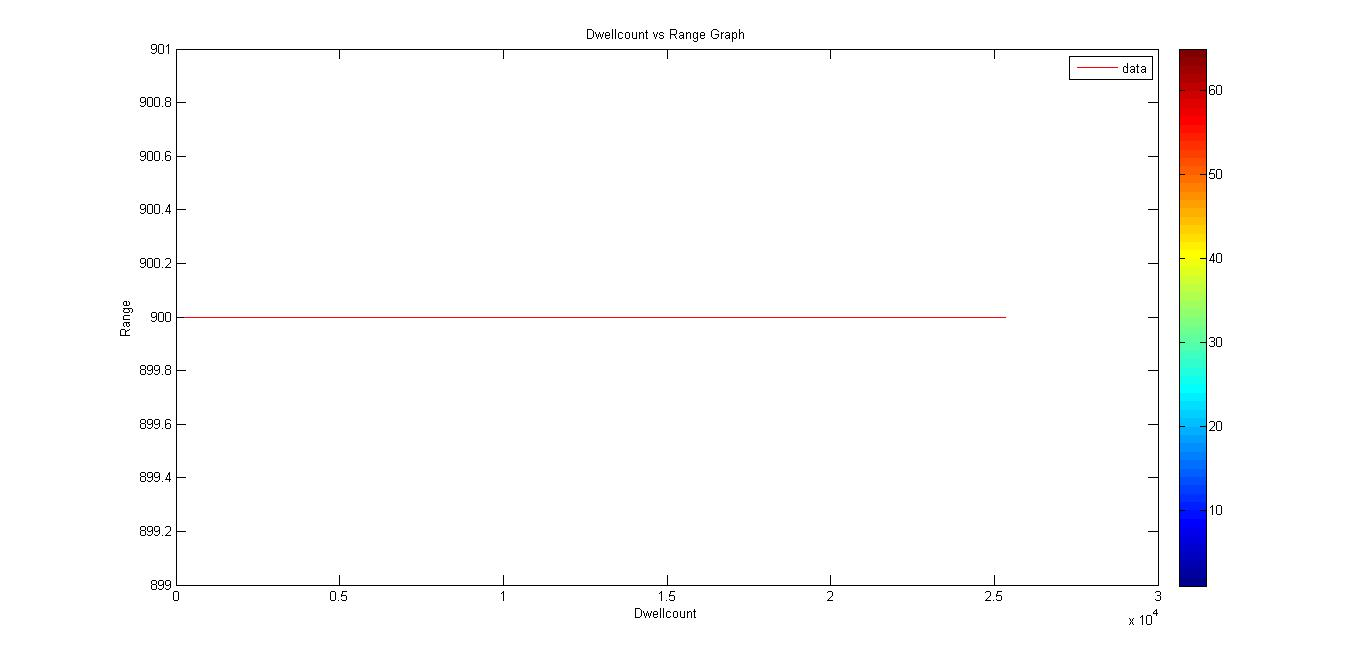
\includegraphics[width=\linewidth]{dwellcount-range(1,25067).jpg}}
  \caption{Plot of dwellcount vs range graph of all the dwellcount from 274 to 25344}
  \label{fig:figure 22}
  \end{figure}
  \begin{tcolorbox}[title =\textbf{Analysis}]
  The graph between dwellcount vs range shows a horizontal straight line which implies, for each dwellcount the range was fixed at 900 which further shows that the simulation was done at fixed range.
  \end{tcolorbox}
  
  \subsection{DWELLCOUNT VS AZIMUTH GRAPH}
  \noindent \textbf{Definition : }\\
   \indent Azimuth $\phi$,$\gamma$ (antenna coordinates) Bearing angle of target relative to Radar system measured clockwise from the perpendicular to the antenna face 
   \begin{figure}[H]
  \centerline{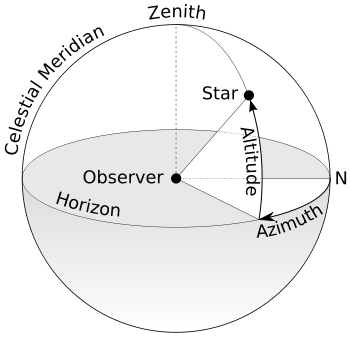
\includegraphics[width=0.4\linewidth]{azimuth.png}}
  \caption{Azimuth is as shown in the figure}
  \label{fig:figure 23}
  \end{figure}
  \textbf{Plot : }The dwellcount and azimuth column is stored in an array variable x and y and plots where made as shown in Figure:
  
  \subsubsection{Plot for dwellcount 274 to 25344}
     \begin{figure}[H]
  \centerline{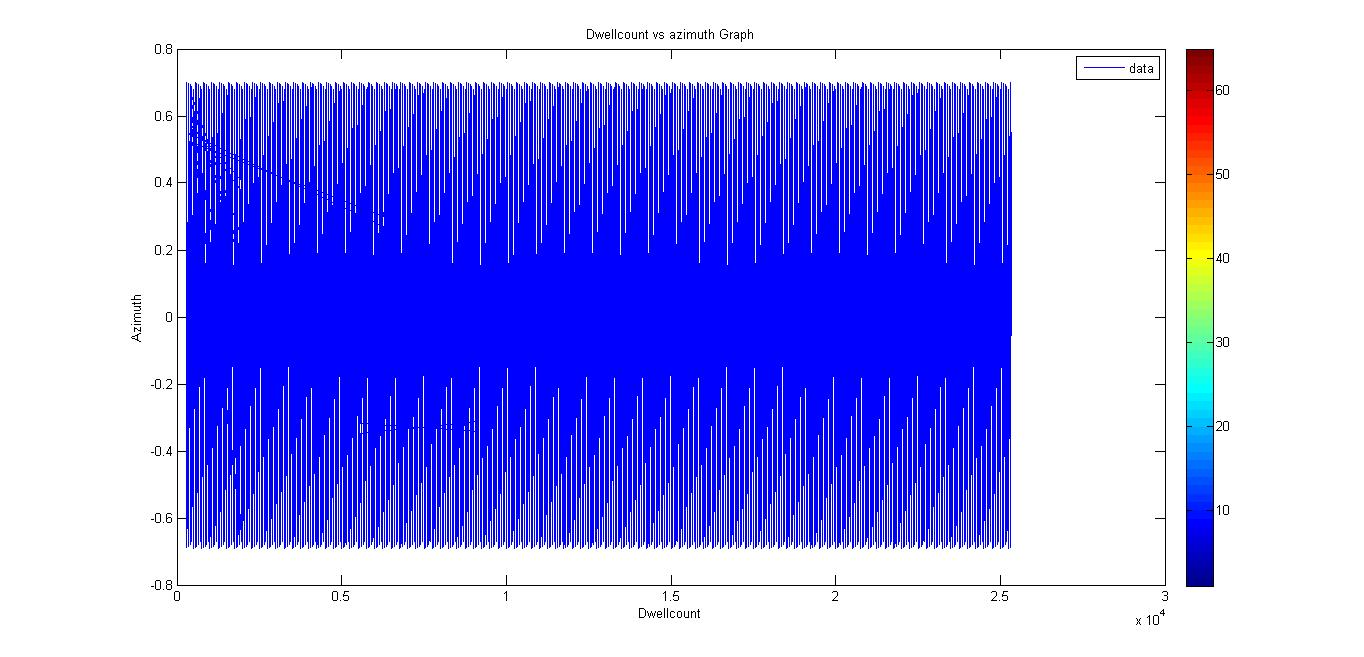
\includegraphics[width=\linewidth]{dwellcount-azimuth(1,25067).jpg}}
  \caption{Plot of dwellcount vs Azimuth graph of all the dwellcount from 274 to 25344}
  \label{fig:figure 23(a)}
  \end{figure}
  \begin{tcolorbox}[title =\textbf{Analysis}]
The graph between dwellcount vs Azimuth shows that the radar was operated priodically between 0.7 to - 0.7 azimuth   .
  \end{tcolorbox}
  
  \subsubsection{Plot for dwellcount 274 to 285}
  \begin{figure}[H]
  \centerline{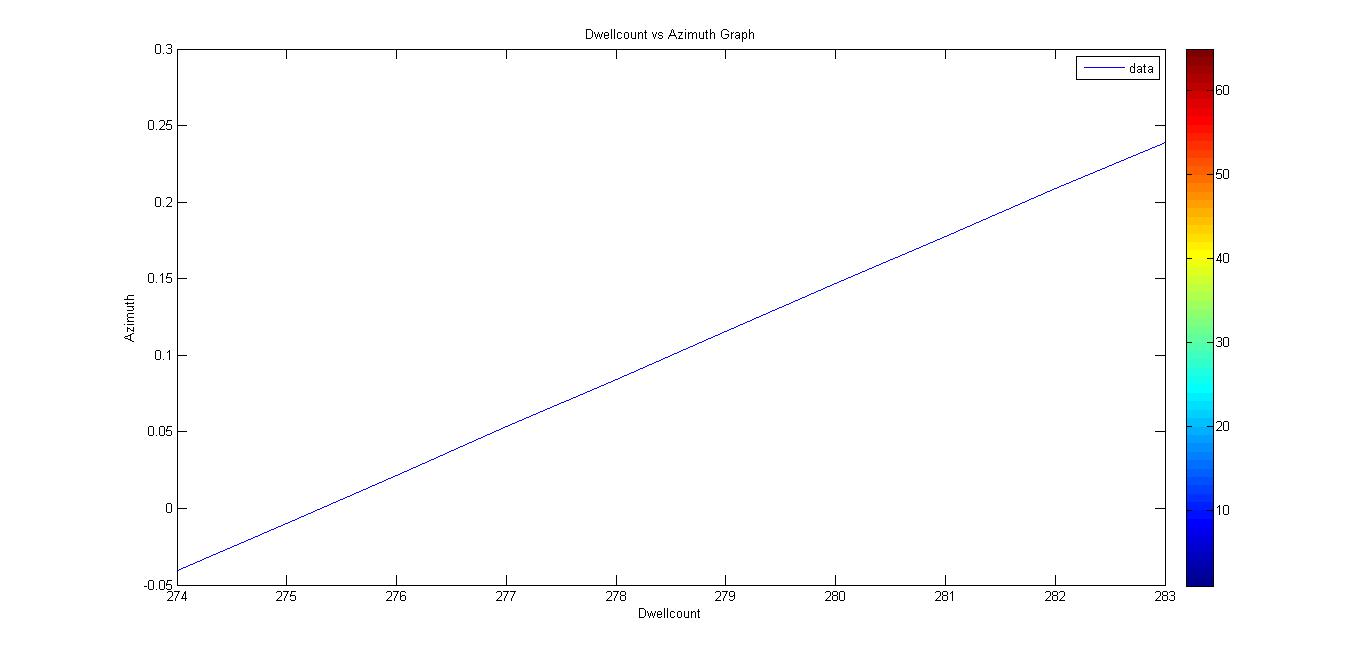
\includegraphics[width=\linewidth]{azimuth(1,10).jpg}}
  \caption{Plot of dwellcount vs Azimuth graph of all the dwellcount from 274 to 25344}
  \label{fig:figure 23(b)}
  \end{figure}
  \begin{tcolorbox}[title =\textbf{Analysis}]
  The graph  between dwellcount vs Azimuth of small interval from 274 to 285 shows sloppy straight curve, which implies that the radar radiates dwells in linear fashion covering all the azimuth angles of operation.
  \end{tcolorbox}
   
   \subsubsection{Plot for dwellcount 4274 to 4295}
   \begin{figure}[H]
  \centerline{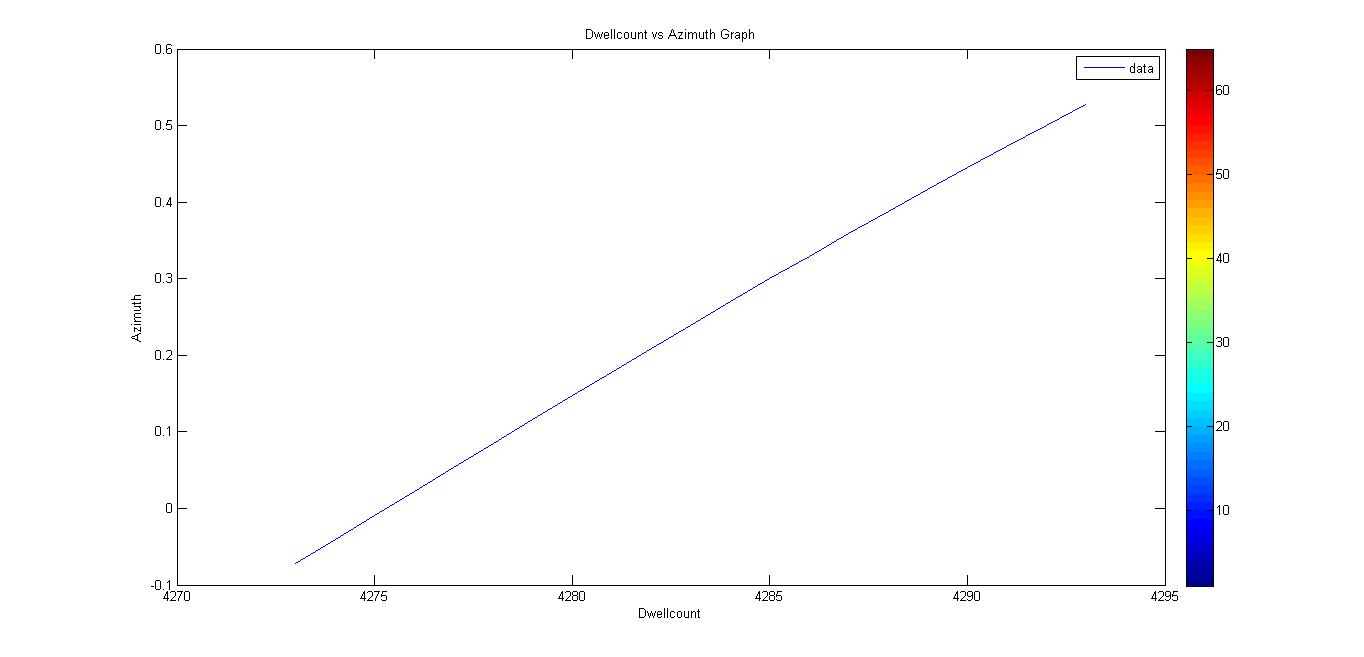
\includegraphics[width=\linewidth]{azimuth(4000,4020).jpg}}
  \caption{Plot of dwellcount vs Azimuth graph of all the dwellcount from 4274 to 4295}
  \label{fig:figure 23(c)}
  \end{figure}
  \begin{tcolorbox}[title =\textbf{Analysis}]
  The graph  between dwellcount vs Azimuth from 4274 to 4295 dwellcout, also shows sloppy straight curve, which implies that the radar radiates dwells in linear fashion covering all the azimuth angles of operation.
  \end{tcolorbox}
  
  
   \subsubsection{Plot for dwellcount 10274 to 10325}
   \begin{figure}[H]
  \centerline{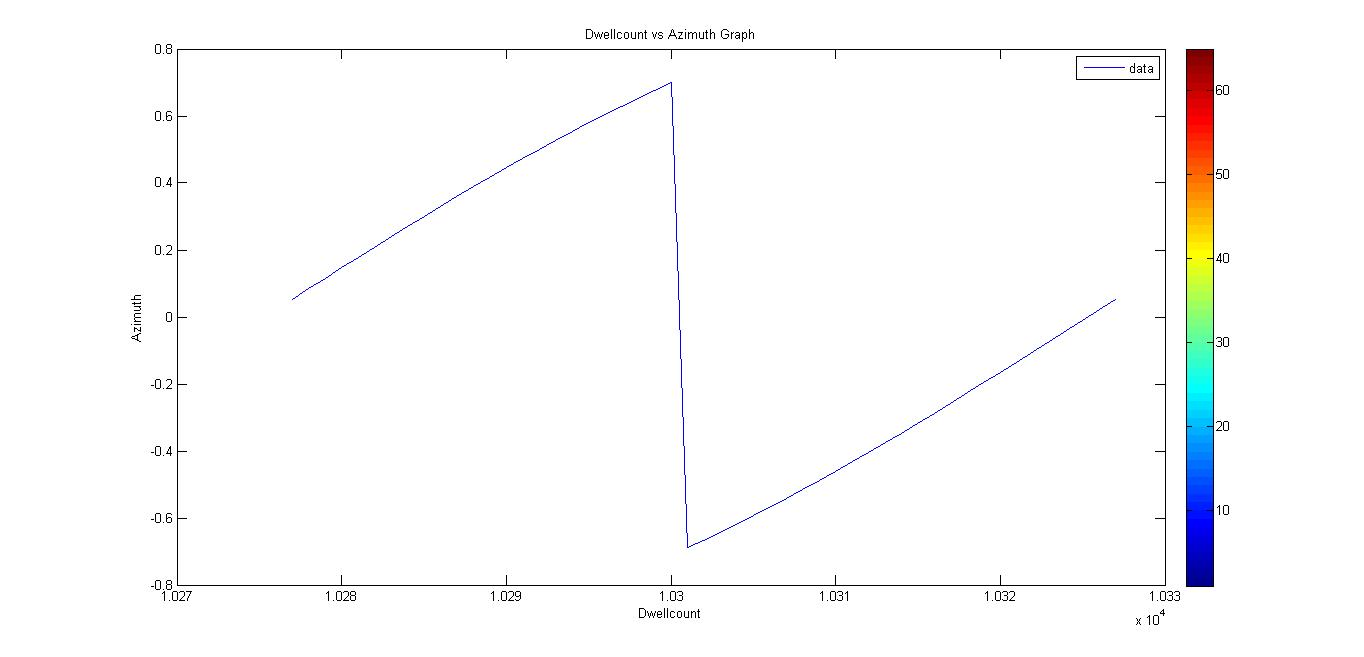
\includegraphics[width=\linewidth]{azimuth(10000,10050).jpg}}
  \caption{Plot of dwellcount vs Azimuth graph of all the dwellcount from 10274 to 10325}
  \label{fig:figure 23(c)}
  \end{figure}
  \begin{tcolorbox}[title =\textbf{Analysis}]
  The graph  between dwellcount vs Azimuth from 10274 to 10325 dwellcout, shows a sudden change in a curve which implies that the radar has started radiating from the -0.7 azimuth.It shows the feature of QRSAM radar as it is different from traditional 360-degree rotating radar, due to its design structure it is capable of radiating dwells in any azimuth.
  \end{tcolorbox}
  
   \subsubsection{Plot for dwellcount 20274 to 20375}
   \begin{figure}[H]
  \centerline{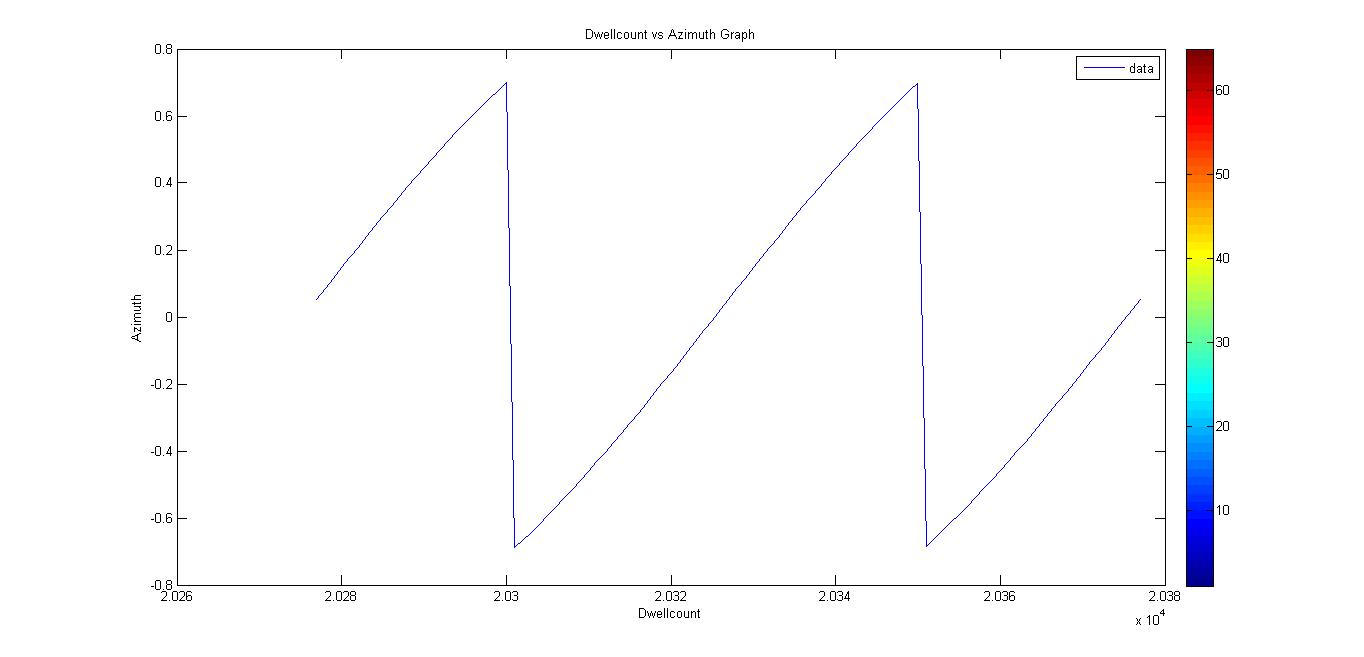
\includegraphics[width=\linewidth]{azimuth(20000,20100).jpg}}
  \caption{Plot of dwellcount vs Azimuth graph of all the dwellcount from 20274 to 20375}
  \label{fig:figure 23(c)}
  \end{figure}
  \begin{tcolorbox}[title =\textbf{Analysis}]
  The graph  between dwellcount vs Azimuth from 20274 to 20375 dwellcout, shows many cycles of peaks and troughs which implies that the radar is continuously radiating dwells from azimuth 0.7 to - 0.7 in regular intervals
  \end{tcolorbox}
  
  The overall analysis of dwellcount vs azimuth graph shows that the radar is sending 50 dwells for each cycle of sweep through 0.7 to - 0.7 azimuth and again starts from 0.7. 
  
\end{document}
